% !TEX root = ../main.tex

% 中英标题:\chapter{中文标题}[英文标题]
\chapter{绪\hspace{1em}论}[Introduction]
% 绪论也需像摘要、目录格式那样空出两个半角字符。

\section{课题背景及研究的目的和意义}[Background, objective and significance of the subject]
\subsection{课题背景}[Background of the subject]
% 正文内容,注意LaTeX分段有两种方法,直接空一行或者使用<\par>
% 默认首行缩进,不需要在代码编辑区手动敲空格
随着人类近年来对河流、湖泊及海洋资源的深入探索,海底地图的精确测绘与海洋生物多样性的科学研究变得愈发关键。对海洋生物与海底资源的探索是海
底研究活动的重要课题,但是鉴于海底环境的极端复杂性和潜在危险性,探测手段正逐步从依赖潜水员直接作业转向利用水下机器人进行远程探测。
相较于光学探测设备在陆地上的广泛应用,在水下探测中光学设备面临着严峻的挑战。光线在水中传播时会被吸收和散射,尤其在浑浊或深水区域,光线
衰减迅速;并且由于水对不同波长光的吸收程度不同,水下图像通常存在色彩失真。
光线在水中传播受限,易受水体中的浑浊物质和微生物吸收和散射影响,导致成像质量显著下降,因此在水下部署可用的基于视觉的状态估计并不简单,
特别是,悬浮颗粒、模糊以及光线和颜色衰减会导致图像特征并不像水面上那样清晰定义。
因此,来自不同基于视觉的状态估计包的结果显示大量异常值,从而导致不准确定位,甚至完全丢失跟踪\cite{rahman2019svin2},使得机器人在水
下环境的感知能力减弱,进而影响机器人的定位和自主导航能力。如图\ref{fig:水下视觉图像}所示,海洋中水下机器人视觉退化严重。

\begin{figure}[!ht]
  % 创建一个图形环境,[!ht] 表示优先将图形放置在“此处”或“页面顶部”
  \setlength{\subfigcapskip}{-1bp}
  % 设置子图标题与图像之间的间距为 -1bp(负值使标题更靠近图像)
  \centering
  % 使图形内容居中对齐
  \begin{minipage}{\textwidth}
    % 创建一个宽度等于文本宽度的迷你页面,用于容纳子图
    \centering
    % 迷你页面内容居中
    \subfigure[\label{fig:image1}]{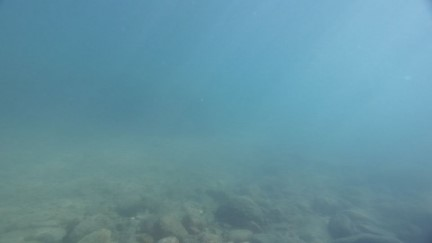
\includegraphics[width=0.48\textwidth]{figures/1.jpg}}
    % 定义第一个子图,标题为“图像1的标题”,插入图片 figures/1.jpg,宽度为文本宽度的 45%
    \hspace{0.5em}
    % 在两个子图之间添加 2em 的水平间距
    \subfigure[\label{fig:image2}]{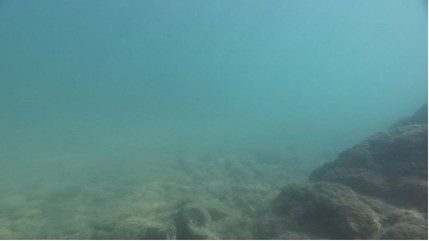
\includegraphics[width=0.48\textwidth]{figures/2.jpg}}
    % 定义第二个子图,标题为“图像2的标题”,插入图片 figures/2.jpg,宽度为文本宽度的 45%
  \end{minipage}
  % \vspace{0.2em}
  % 在图形与下方内容之间添加 0.2em 的垂直间距
  \caption{水下视觉图像}
  \label{fig:水下视觉图像} % 为整个图形添加标签
\end{figure}

相比之下,声纳技术在水下探测领域展现出了显著的优势。其核心在于声波能够在水中实现远距离的有效传播,这一特性使得声纳系统
能够覆盖更广阔的水域范围,进行更为全面的探测;尤为重要的是,声纳受水体浑浊度的干扰较小,即便是在水质较差、
能见度较低的环境中,依然能保持较高的精度和稳定性。
因此,声纳技术成为了水下探测领域的优选方案,为水下作业和科研探索提供了强有力的支持,大多数水下机器人均装备有声纳等声学
传感器,可以更好地完成海底基础设施检查、船体检查\cite{kaess2010towards}和海底测量和测深\cite{fallon2011efficient}等任务。

\subsection{研究的目的和意义}

水下声学环境的复杂性源于多种因素,使得声波在传播过程中面临诸多挑战。首先,多路径效应是声波在水中传播时常遇到的现象,声波会因为水下物体的反射和折射而产生
多条传播路径,这些路径在抵达接收器时可能会相互干扰,导致信号失真。其次,近场干扰进一步增加了这一复杂性。在近距离内,声波的传播受周围环境的影响显著,声波
可能会因为水流、温度梯度和盐度变化等因素而产生波动,影响传感器的准确性。除了这些物理现象,水下声学环境中还存在着多种来源和类型的噪声干扰。来自船只、海洋
生物、波浪以及人类活动等的噪声,都会对传感器收集到的原始数据产生显著影响。
这些噪声不仅会掩盖目标信号,还可能与目标信号混合,进一步复杂化信号处理过程。因此,传感器常常难以提取有效信息,导致数据质量下降。同时由于受到声波多路径反
射的影响,导致真实声纳信号周围产生伪影\cite{cervenka2002sidescan},从而极大地增加了从这些数据中准确提取特征、识别对象或界定边界的难度。
现有声纳图像去噪方法主要分为传统滤波类与深度学习类两大类。关于传统的去噪方法,在面对水下声纳图像特有的噪声模式时,往往效果有限,无法有效恢复出清晰高质量的
图像信息,如图\ref{fig:传统去噪方法效果图}所示,经过传统滤波处理后,仍存在大量噪声,可见传统滤波处理算法的鲁棒性较差。而深度学习的方法依赖大规模配对数据
进行监督训练,而真实水下环境中难以获得与噪声图像严格对应的“干净”样本,导致模型泛化性不足,难以适用于不同声纳设备与环境条件。


\begin{figure}[!ht]
  \centering
  % 设置边框与图像之间的间距(可调,建议 1pt ~ 3pt)
  \setlength{\fboxsep}{2pt}
  \setlength{\fboxrule}{1pt}  % 边框粗细

  % ---- 保存第一张图的“标准尺寸盒子”(不含边框)----
  \newsavebox{\standardimage}
  \savebox{\standardimage}{%
    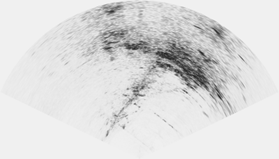
\includegraphics[width=0.48\textwidth]{figures/声纳原始图像.png}%
  }

  % --- 第一行 ---
  \begin{minipage}{\textwidth}
    \centering
    \subfigure[声纳原始图像\label{fig:a}]{%
      \fbox{\usebox{\standardimage}}% 加边框
    }\hspace{0.5em}
    \subfigure[小波变换去噪后图像\label{fig:b}]{%
      \fbox{%
        \resizebox{!}{\ht\standardimage}{%
          \resizebox{\wd\standardimage}{!}{%
            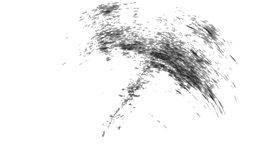
\includegraphics{figures/小波变换.png}%
          }%
        }%
      }%
    }
  \end{minipage}

  \vskip 1em  % 两行之间间距

  % --- 第二行 ---
  \begin{minipage}{\textwidth}
    \centering
    \subfigure[Lee滤波器去噪后图像\label{fig:c}]{%
      \fbox{%
        \resizebox{!}{\ht\standardimage}{%
          \resizebox{\wd\standardimage}{!}{%
            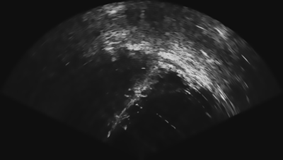
\includegraphics{figures/Lee滤波器.png}%
          }%
        }%
      }%
    }\hspace{0.5em}
    \subfigure[各向异性去噪后图像\label{fig:d}]{%
      \fbox{%
        \resizebox{!}{\ht\standardimage}{%
          \resizebox{\wd\standardimage}{!}{%
            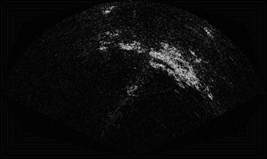
\includegraphics{figures/各向异性.png}%
          }%
        }%
      }%
    }
  \end{minipage}

  \caption{传统去噪方法效果图}
  \label{fig:传统去噪方法效果图}
\end{figure}

针对上述问题,本研究提出一种基于生成对抗网络的渐进式声纳图像去噪框架 SonarGAN,通过结合非配对学习与成对约束,实现多源噪声的联合抑制与结构信息的自适应保
持。该方法不仅突破了传统监督方法对配对数据的依赖,还在多种声纳类型及真实水下场景中表现出优异的泛化性能。此外,本文进一步探索了去噪图像在三维场景重建中的
应用价值,验证了声纳图像质量提升对下游任务性能提升的直接促进作用。

本研究为前视声纳图像提供了一种高效的去噪方案,在应用上提升了声纳图像在三维重建与水下感知任务中的可用性与鲁棒性,对智能水下机器人、自主探索与海洋健侧等领
域具有一定的工程应用价值与推广意义。


\section{国内外研究现状}

水下机器人是在水下作业的一种机器人,随着各国对海洋探索的竞争,水下机器人也在快速发展,加之海洋中油田、天然气资源勘探的发现,使得研发智能化水下机器人变得
更加重要,更加迫切。自主水下航行器(AUV)实现了水下作业平台的小巧化、智能化,通过线缆与陆地进行控制和通信,提高了水下作业的灵活度,也更加适用于未知海域
的探索,也可以搭配不同的组件,如机械臂,声纳等,完成不同的特定功能。

\subsection{水下机器人领域研究现状}

通常,水下机器人可分为自主水下机器人(Autonomous Underwater Vehicle, AUV)和遥控水下机器人(Remotely Operated Vehicle, ROV)。AUV自带能源,可以自
主航行,能够执行大范围探测任务,但作业时间、数据实时性、作业能力有限。ROV依靠脐带电缆提供动力,水下作业时间长,能够实现数据实时传输,作业能力较强,但作
业范围有限。近年来发展的混合式水下机器人——自主遥控水下机器人(Autonomous \& Remotely Operated Vehicle, ARV)结合了AUV和ROV的优点,自带能源,通过光
纤微缆实现数据实时传输,既可实现较大范围探测,又可实现水下定点精细观测及轻作业。相关水下机器人如图\ref{fig:rov-comparison}所示。

\begin{figure}[!ht]
  \setlength{\subfigcapskip}{-1bp}
  \centering
  % ---- 保存第一张图的“标准尺寸盒子” ----
  \newsavebox{\standardrov}
  \savebox{\standardrov}{%
    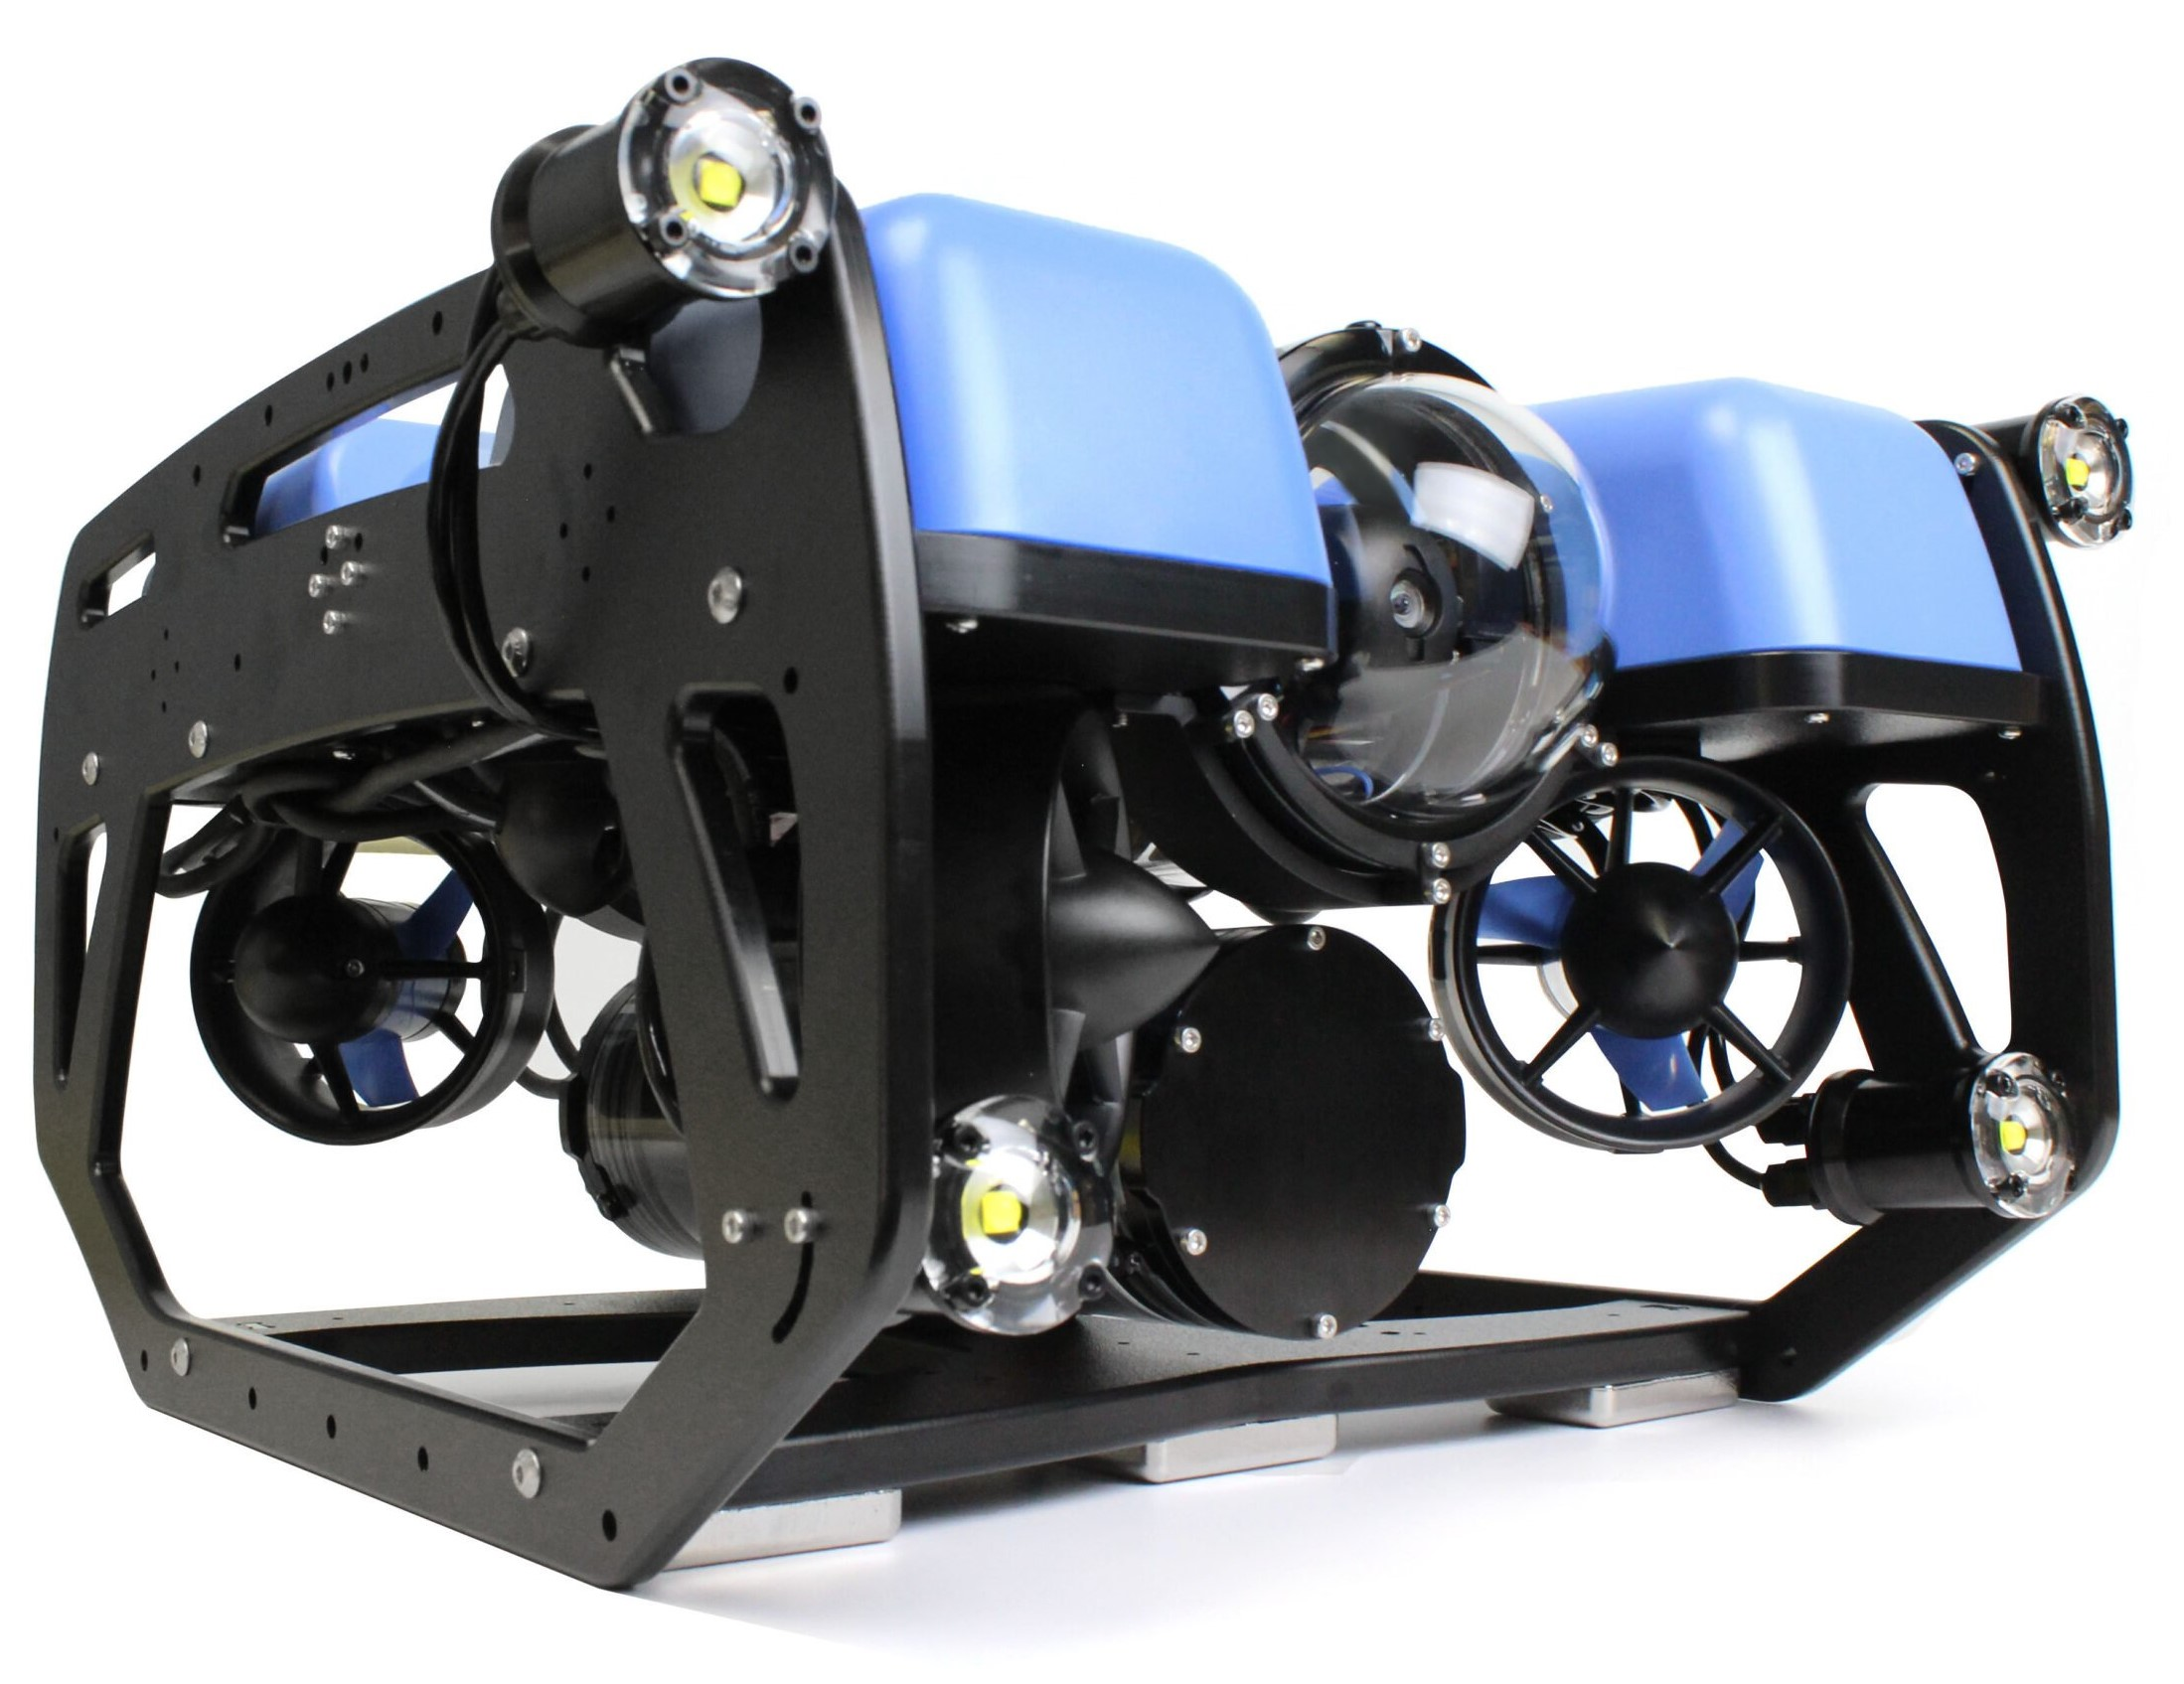
\includegraphics[width=0.42\textwidth]{figures/bluerov2.jpg}%
  }
  % --- 两张图并排 ---
  \begin{minipage}{\textwidth}
    \centering
    \subfigure[BlueRov2\label{fig:rov-a}]{%
      \usebox{\standardrov}% 第一张:原始尺寸
    }\hspace{0.8em}
    \subfigure[蛟龙号\label{fig:rov-b}]{%
      \resizebox{!}{\ht\standardrov}{% 强制等高
        \resizebox{\wd\standardrov}{!}{% 强制等宽
          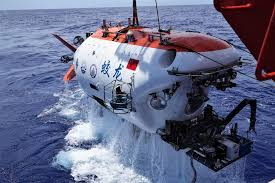
\includegraphics{figures/蛟龙号.jpg}%
        }%
      }%
    }
  \end{minipage}

  \caption{BlueROV2 与蛟龙号水下机器人}
  \label{fig:rov-comparison}
\end{figure}

国外方面,国外水下机器人研究已有近70年的历史。以美国为代表的西方发达国家,先后研发了ROV、AUV、ARV以及水下滑翔机等多种不同类型的水下机器人,主要用于深海
资源勘查、海洋科学考察和军事应用等领域。20世纪50年代,遥控水下机器人首次用于回收鱼雷。之后在寻求降低成本和减轻操作员风险的过程中,自主遥控水下机器人得到
了发展。基于BlueRov2 ROV开发的AUV节省了大量时间,并且简化了部署,从而降低了运营成本。Nessie-V是一款6自由度研究型AUV,由赫瑞瓦特大学海洋系统实验室开发
,用于重点检查和自主任务的研究。Girona500,这是一种具有可重新配置有效负载和推进系统的自主遥控水下机器人。

国内方面,2008年,中国科学院沈阳自动化研究所完成了“北极”ARV的研制,2009年,中国船舶重工集团公司第702研究所完成了“海筝I型”ARV原理样机的研制,并后续投入
使用。2013 年,上海海事大学完成了“海事一号”ARV的研制,可以应用于浅海渔业监测,水下搜救等作业任务。2020年,由中国科学院沈阳自动化研究所牵头,联合中国10
余家优势单位共同研制的“海斗一号”全海深自主潜水器完成了万米海底试验验证。


\subsection{声纳图像去噪研究现状}

早期的声纳图像去噪研究主要针对于散斑噪声(speckle noise)展开,经典的滤波算法如Lee滤波器、Kuan滤波器和Frost滤波器等最初是为合成孔径声纳(Synthetic Aperture Sonar, SAS)
图像设计的~\cite{mascarenhas1997overview}。这些方法基于乘性散斑噪声模型(multiplicative speckle model)来估计局部区域的统计特性,从而实现噪声抑制,
但模型的不精确性经常导致角点等精细结构的损失。为改善这一问题,Lopes等人提出了一种基于双阈值变异系数(dual-threshold coefficient of variation)的自适
应方法,从而在去噪的同时更好地保留边缘信息~\cite{lopes2002adaptive}。随后,一些通用的图像去噪方法,如小波变换(wavelet transform)~\cite{chang2000adaptive}
、非局部均值法(non-local means)~\cite{buades2005non}以及BM3D算法~\cite{dabov2007image}也被应用于声纳图像去噪中,在保留细节的同时提供了更强的噪声抑制
效果。尽管这些方法取得了一定进展,但是传统方法在处理前视声纳图像中的结构性噪声(structural noise)时仍显不足,例如条纹状伪影与固定点伪影等问题依然难以有效解决。

随着深度学习的发展,卷积神经网络已经被广泛应用于声纳图像去噪任务中。Ji等人提出了一种基于Noise2Void的自监督去噪方法,能够有效去除高斯噪声和散斑噪声~\cite{ji2025sonar};Si
等人提出WTCRNet,将小波变换与对比正则化相结合,用于前视声纳图像去噪~\cite{si2024wtcrnet}。此外,结合卷积神经网络(CNN)与自注意力变换网络(Transformer)的盲去噪模型 SCUNet 也被引入到
声纳图像处理中~\cite{zhang2023practical}。最近Vishwakarma提出一种基于卷积稀疏表示(convolutional sparse representation)的去噪与修复方法,可有效保留
边缘与纹理细节~\cite{vishwakarma2023denoising}。

生成对抗网络(Generative Adversarial Networks, GANs)在声纳去噪领域同样展现出巨大潜力。典型的非配对学习框架包括UIDNet~\cite{hong2020end}、UNIT~\cite{liu2017unsupervised}、
CUT~\cite{park2020contrastive}、StillGAN~\cite{ma2021structure}与DRGAN~\cite{huang2020noise},它们均通过对抗训练提升了图像去噪的有效性。
在声纳场景中,Zhao等人提出了NCD-GAN,通过联合对比学习实现了非配对去噪~\cite{zhao2023unpaired};Lin等人基于条件生成对抗网络从前视声纳图像中生成噪声掩膜以
滤除噪声~\cite{lin2023conditional};Zhou 等人提出的STGAN将生成对抗网络与自注意力变换网络(Transformer)结合,用于抑制散斑噪声~\cite{zhou2023stgan}。
这些方法在复杂噪声环境下的表现优于传统算法,但仍面临训练不稳定与模式坍塌(mode collapse)等问题。

近年来,扩散模型(Diffusion Models)也被广泛应用于声纳图像去噪任务。Ho等人提出了DDPM(Denoising Diffusion Probabilistic Model),为扩散模型奠定了
理论基础~\cite{ho2020denoising}。Smith等人将扩散模型用于声纳超分辨率任务中,有效缓解了条纹噪声问题~\cite{bryan2025diffusion};Wang等人将DDPM应用于
侧扫声纳(Side-scan Sonar)去噪,在真实数据集上获得了显著性能提升~\cite{yang2023side}。然而,尽管扩散模型的去噪效果优异,其训练和推理成本较高,因而不适用于
实时声纳图像去噪任务中。

\section{本文的主要研究内容}[Main research contents of this subject]

近年来,随着水下机器人技术的快速发展,环境感知与重建已成为自主作业系统的关键环节。前视声纳(Forward-Looking Sonar, FLS)作为一种重要的水下成像传感器,能够在
低能见度、强浑浊等光学图像无法工作的环境下提供高分辨率图像信息,因此在水下探测、定位和导航任务中得到了广泛应用。然而,由于声波在传播过程中受到多路径反射、散射
以及硬件噪声等影响,声纳图像常常受到散斑噪声、旁瓣噪声和结构性噪声等多种干扰。这些噪声不仅严重降低图像对比度与分辨率,还导致目标边界模糊,显著影响后续的目标识
别、三维重建与自主导航等任务。针对上述问题,本文提出了一种基于生成对抗网络的多阶段声纳图像去噪框架SonarGAN,旨在实现多类型噪声的联合抑制与结构信息的有效保持。
本文的主要研究内容包括以下几个部分:

\textbf{1.基于无配对数据的初步声纳去噪。}针对水下声纳图像难以获取真实配对(噪声——干净)样本的问题,本文首先设计了一个无监督的初步去噪框架。该阶段以循环一致性
对抗网络(Cycle-Consistent Adversarial Networks,CycleGAN)\cite{zhu2017unpaired}为基础,通过构建噪声域与干净域之间的循环一致性约束,实现不同域之间的特征
迁移与映射。本阶段主要针对随机噪声(如散斑噪声、旁瓣噪声)进行初步抑制,在不依赖配对样本的前提下获得具有较高结构一致性的去噪结果。本阶段中引入感知损失,以在深层
特征空间上约束生成器保持目标的边缘与纹理语义。为了避免传统CycleGAN容易出现的伪影与纹理漂移问题,本文在生成器中嵌入了自注意力模块(Self-Attention Module),
以增强模型的全局感知能力,从而在早期阶段实现噪声的有效压制与纹理信息的保持,为后续阶段提供高质量的特征先验。

\textbf{2.基于配对数据的结构性噪声抑制。}为了进一步去除结构性噪声并提升图像细节质量,本文在第二阶段引入了基于条件生成对抗网络(Conditional Generative Adversarial Networks, cGAN)
\cite{isola2017image}的精细去噪模块。该阶段利用显式的配对训练集:通过将实测的纯噪声图像叠加到仿真得到的无噪图像上,得到带结构噪声的合成样本对,进行训练.通过显式学习声纳成像机制中结构
性噪声的分布特征,增强网络对目标边界及结构性噪声的敏感性。在本阶段得到的生成器能有效识别并剔除稳定存在的结构性干扰,为第三阶段提供结构先验。

\textbf{3.联合约束去噪。}在第三阶段,本文提出了一个多阶段融合与联合约束机制,对前两个阶段的输出结果进行统一优化与精修。该阶段通过设计显著性掩模约束,在像素层面
实现噪声抑制与结构保持的动态平衡。掩模由网络自适应生成,用于区分目标区域与背景噪声区域,使模型在噪声区域增强抑制能力,而在目标区域重点保留纹理细节。同时,本文在
损失函数中引入对抗约束与特征一致性约束,实现了从全局结构到局部细节的多层次优化。经本阶段融合后,SonarGAN 能够在多类型噪声共存的复杂水下环境中稳定实现高质量去噪
与结构保真,显著提升了模型的鲁棒性与泛化能力。

\textbf{4.实验设计与性能验证。}为验证所提出方法的有效性与通用性,本文设计并开展了两类实验:去噪性能评估实验与三维重建验证实验。

在去噪性能评估部分,本文分别在仿真数据集与真实声纳数据集上对比了SonarGAN与多种主流去噪方法的性能表现,包括传统滤波方法(Lee、BM3D等)、深度学习方法(DnCNN、S
CUNet等)以及多种生成对抗网络框架(CycleGAN、UNIT、CUT、StillGAN等)。仿真实验采用虚拟仿真环境生成的噪声自由图像,并结合多种声纳的实测噪声进行合成含噪声图像,
以获得多样化的测试样本。真实实验使用同类声纳在实验水池、河流环境以及港口码头中采集的数据,综合评估模型在不同噪声分布下的表现。本文除了采用PSNR、SSIM、LPIPS等常
规指标,还提出了一种新的基于Kullback–Leibler(KL)散度\cite{kullback1951information}的统计分布差异指标对去噪性能进行量化评估,并设计了基于平均残差图像的空
间一致性度量方法,以进一步衡量模型的噪声去除和目标物体保留能力。实验结果表明,SonarGAN在多种噪声类型与不同声纳设备下均取得优异的去噪效果,能够有效去除结构性噪
声并保持目标细节。同时,本文通过跨域泛化实验验证了模型的稳健性,即直接将河流数据上训练的模型应用于实验水池数据,仍能获得理想的去噪结果。

在三维重建验证部分,本文进一步评估了去噪质量对水下重建任务的促进作用。通过将去噪前后的声纳图像输入至基于声波传播建模的三维重建算法中,比较重建点云的稠密度、表面
平滑性与几何一致性等指标,结果显示经SonarGAN去噪后的声纳图像在纹理一致性与深度恢复方面均显著优于原始图像和多种对比算法的去噪后声纳图像,证明了所提方法在水下
任务中的实用价值。


